\chapter{绪论}
\label{cha:intro}

\section{研究背景}

\emph{嵌入式系统}~\cite{heath2002embedded} 最早出现在六十年代,其产生是为了减少搭载系统的体积重量以及降低成本。作为计算资源的成本高昂的计算机逐步被成本相对低廉的微处理器系统替换,导致设备不仅变得小型化、低价格,同时处理能力以及功能也不断提高。这些变化使得七八十年代时期,民用电子、消费类电子等行业得到了快速发展并大规模兴起。从工业 2.0 时代开始的自动化、电力驱动的大规模工业生产中,早期的嵌入式系统开始大量投入使用。到现在的工业3.0时代以及2013年德国提出的工业4.0,以信息化、智能化、自动化、网络化作为核心,数字化产品以及产品生产制造过程,其全生命周期都将依赖于电子信息而产生的新工业模式。在这中间,嵌入式系统的不断强大将为工业的进程提供技术支撑,以加快工业 4.0 在全领域的普及。

最早,不同的嵌入式系统承载不同功能,其设计是为特定系统、特定任务而定制的,大多数嵌入式系统都是功能单一的系统。在发展过程中,嵌入式系统的处理单元逐渐变得强大(如现在的 ARM、PowerPC、MIPS 等),外围设备、硬件资源越来越丰富,使其可以承担更多复杂的处理任务,并具有了通用性、架构可移植的特点。在嵌入式系统硬件能力提升的基础上,除了为硬件系统开发固件外,Linux、MS-DOS,以及专为嵌入式系统开发的实时操作系统 VxWorks 等操作系统的加入,可以完成系统设备的协调调度、资源监管等任务,并且使得开发运行针对应用需求的用户控制界面和具有更多功能的应用软件成为可能。 

除消费类电子产品外,嵌入式系统在民用、军用大型设备中的作用同样重要。在航空领域中,民用航空飞机的机载电子设备功能越发强大,系统架构也越发复杂。飞行控制系统、导航系统、通信系统、雷达系统、环境控制系统,以及各终端传感器系统都搭载了嵌入式系统来对其进行控制,并完成计算、存储、传输等以支持飞控、通信、导航等高级任务。其中系统异步、并发、调度、实时等问题引起的不确定性都是影响系统正常工作、影响飞行安全的重要因素。安全性是民用飞机的重要属性,系统安全性的设计、验证以及管理贯穿飞行器整个生命周期。有 ARP4754~\cite{ARP4754A}、ARP4761~\cite{ARP4761} 来指导飞行器系统的安全性设计,以及 DO-178C、DO-254 来指导符合安全性等级的软件、硬件设计。其中嵌入式系统的硬件要满足安全性设计中对应的可靠性需求,而固件及软件系统则要满足对应的软件验证需求。如飞控系统的安全性等级为 A 级,其涉及的嵌入式系统硬件设备要满足安全性保障等级为 A 的设计、测试、验证流程;对于其系统软件,则要求其设计及验证过程中必须使用严格的\emph{形式化方法} 对其安全等级进行保障。其它安全攸关的系统,如轨道运输、海洋运输都有相应的安全性保障需求。嵌入式系统硬件设计验证方法早已比较成熟,但是软件的形式化设计验证方法相对于硬件起步较晚。随着嵌入式系统软件发展的加快,针对嵌入式系统软件的形式化设计与验证存在迫切需求。在嵌入式系统的设计与开发过程中,硬件与软件往往是难以分开单独设计的,因为其软件及固件开发的专用性,互相影响程度很深。所以一种基于形式化方法的、可以同时对硬件及软件系统进行验证的方法亟待研究。

形式化建模与验证方法的基本流程如图~\ref{f:modeling-and-verification} 所示。建模人员需要先对目标系统进行手工或自动建模,得到系统的行为模型。针对系统的行为模型,验证人员再根据其关心的系统属性,利用相应的验证技术,如\emph{模型检测}~\cite{clarke1999model}(model checking)、\emph{定理证明}~\cite{DBLP:books/daglib/0070484}(theorem proving)等,及其相应的工具对系统模型进行形式化验证,从而得到针对属性的验证结果。根据验证结果,开发人员可以对目标系统进行修改或调整。在整个流程中,形式化的系统模型作为连接建模过程和验证过程的桥梁,对建模的难易程度、精确程度及验证的效果都起着至关重要的作用,是整个形式化建模验证方法的基础。

\begin{figure}[ht]
\centering
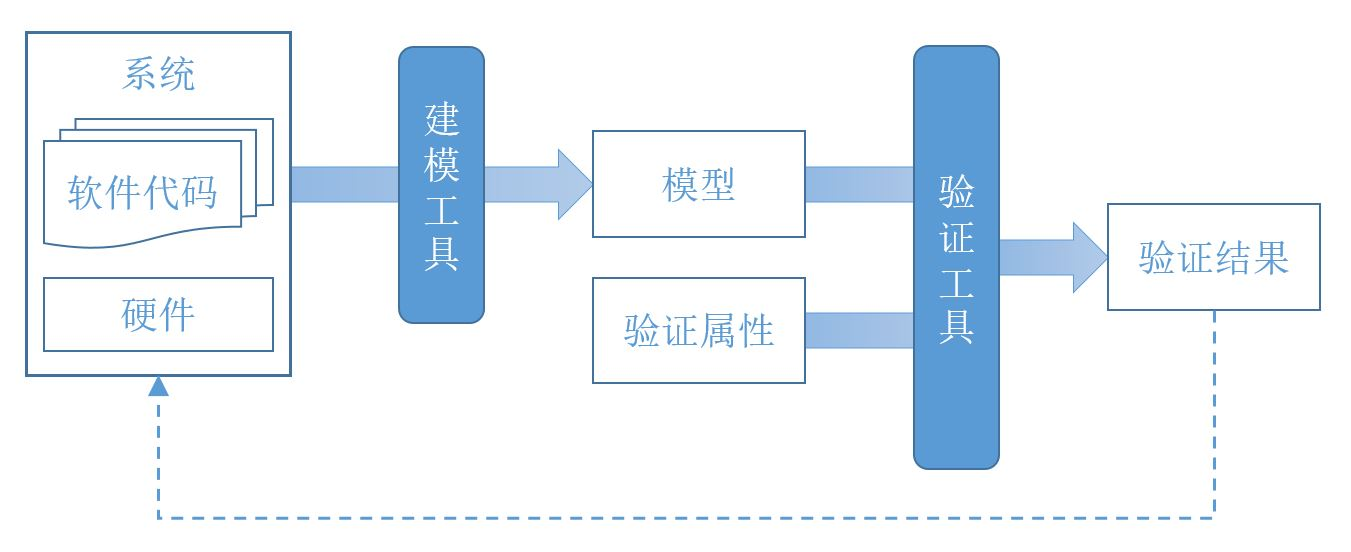
\includegraphics[width=\textwidth]{modeling-and-verification.jpg}
\caption{形式化建模与验证基本流程}
\label{f:modeling-and-verification}
\end{figure}

在种类繁多的嵌入式系统中,存在一类系统,它们与环境存在频繁的交互:它们通过输入设备(如传感器等)从环境接收周期性或非周期性的输入,系统对这些输入进行处理,然后通过输出设备(如执行器等)将处理结果反馈到环境中。这类系统被称作\emph{反应式系统}~\cite{DBLP:conf/iccd/Koopman96,DBLP:books/daglib/0010292}(reactive system)。大部分嵌入式系统都是反应式的:小到我们身边的消费类电子产品(如智能穿戴设备),大到交通运输系统(如第~\ref{s:TO} 小节讨论的机车控制系统)。由于反应式系统的输入不是单一的数值或事件,而是一个可能无穷的输入序列,这一显著特征从两个方面对形式化建模验证所使用的形式化模型提出了要求。
\begin{enumerate}
\item 
表达能力,即建模能力。随着现代嵌入式系统处理单元计算能力的提高,在硬件条件允许的情况下,多线程技术越来越多地被应用到反应式系统中~\cite{DBLP:conf/codes/GerndtE97,DBLP:journals/sigsoft/White11,DBLP:journals/tc/LiH12}。这一方面给系统引入了更多的并发性,要求形式化模型可以对并发行为进行描述;另一方面也要求形式化模型可以对线程的创建、释放等行为进行描述。出于对可组合性和层次化的考虑,线程一般被看作系统中的组件进行建模,于是线程的动态创建与释放行为要求形式化模型具有对系统结构动态变化的描述能力。
\item
验证能力。无穷的输入序列以及多线程带来的并发性使传统的模型检测技术可能面临状态空间爆炸的问题~\cite{DBLP:conf/ac/Valmari96}。因此,对反应式系统的形式化验证要求所使用的模型支持能解决状态空间爆炸的形式化验证技术,如定理证明。
\end{enumerate}

在下一小节中,我们将从上述两个方面对主流建模方法及形式化模型进行介绍和对比。

\section{研究现状}

嵌入式系统的建模方法不胜枚举,根据其描述对象的不同,可以建立架构模型、状态模型、数据模型等。它们分别以不同角度去描述嵌入式系统,用仿真、测试、形式化验证等方法保证系统的正确性、有效性、可靠性等多方面重要属性,特别是对安全攸关系统的设计、验证与运行提供有力支持。如上一节提到,嵌入式系统在众多安全攸关系统(如航空航天飞行器、铁路、核电站、医疗、保密系统等)中扮演着重要的角色。自 1990 年起,已有多份统计以研究报告与论文的形式指出形式化方法在工业领域中所取得的突出成果。2009 年英国约克大学的 Jim Woodcock 统计得到\cite{DBLP:journals/csur/WoodcockLBF09}:在工业应用中,对比只依赖于测试验证的工程开发,基于形式化建模与验证的工程项目有 92\% 得到了产品品质的提升,体现在更少的故障、正确性的提升、设计能力提升等多方面。

在这些形式化方法中,有些用抽象的形式化规约(specification)避免模型中的二义性,从而保证设计质量,如VDM~\cite{DBLP:conf/fm/1978}、Z~\cite{DBLP:books/daglib/0067866} 等。有些用状态模型描述系统行为特性,模型本身能够采用静态分析与模型执行来进行验证,如Petri网~\cite{murata1989}、自动机~\cite{DBLP:books/aw/HopcroftU79} 等。 

\emph{有限状态机}~\cite{minsky1967computation}(FSM)是面向系统状态最基本的模型,被控制系统广泛地应用。但对于功能、架构复杂的嵌入式系统,有限状态机缺乏对其并发性、实时性等方面的支持。所以有限状态机有多种扩展形式:支持并发性的\emph{层次化并发有限状态机}~\cite{DBLP:journals/scp/Harel87}(Hierarchical Concurrent FSM,HCFSM)以及支持时间的\emph{时间自动机}~\cite{DBLP:journals/tcs/AlurD94,DBLP:conf/cav/Alur99}(timed automata)。HCFSM可将一个状态组视为一个状态,状态组之间通过全局变量进行通信,可以用于描述多组件的、并发的控制系统。时间自动机作为有限状态机的另一个变种,增加对状态转移过程中时间因素的描述,变迁上标记的是该状态转移发生的时间约束,从而可以满足对实时系统时间分析的需求。然而,自动机及其扩展模型的模型结构是静态的,因此无法对系统结构的动态变化进行表达。

\textsc{Uppaal2k}~\cite{larsen1999uppaal2k},作为 \textsc{Uppaal}~\cite{DBLP:journals/sttt/LarsenPY97} 的后继工具,提供了对时间系统的建模、仿真以及验证功能,适用于对具有共享变量、通道通信的系统进行描述。\textsc{Uppaal2k} 支持对时间自动机图形化的建模、动态仿真以及模型检测等功能,可以进行有界活性检测、死锁检测、验证使用TCTL~\cite{DBLP:journals/logcom/BouchenebGR09}(Timed Computation Tree Logic)表达式描述的多种性质,不支持定理证明技术。

\emph{Petri 网}~\cite{murata1989} 的研究与应用相当广泛。由于对异步并发系统描述上的优势,Petri 网在实时系统、协议验证、硬件设计、制造过程、商业管理等众多领域中均发挥了作用~\cite{DBLP:journals/isci/KheldounBI17,DBLP:journals/jwe/XuPW17,DBLP:journals/tmc/ZhangAYM16,DBLP:conf/ACISicis/SalahBK15}。在实时嵌入式系统的应用中,Petri 网为描述待验证系统的异步、并发性、不确定性等多种特性提供了有效工具。虽然 Petri 网的网络结构是静态的,即它的三要素——库所、变迁以及有向弧不会发生改变,但由于 Petri 网的令牌(token)数量动态可变,且 Petri 网的状态由令牌分布决定,因此它可用于描述对象系统的结构变化。为了扩展标准 Petri 网的适应性,Petri 网衍生出多种变种,如着色 Petri 网~\cite{DBLP:series/eatcs/Jensen97}(Colored Petri Net,CPN)、对象 Petri 网~\cite{DBLP:conf/apn/Lakos95}(object Petri net)、混合 Petri 网~\cite{david2010discrete}(hybrid Petri net),
\hide{随机Petri网(stochastic Petri net),}
以及多种时间相关的 Petri 网,如 Time Petri Net~\cite{DBLP:journals/tse/BerthomieuD91}(TPN)、Timed Petri Net~\cite{DBLP:conf/isca/Zuberek80}(TdPN)、Timing Constraint Petri Net~\cite{DBLP:journals/tse/TsaiYC95}(TCPN),以适用于不同的应用需求。

\hide{
在以嵌入式实时系统为验证对象时,时间是最重要的因素之一,时间自动机以及各类时间 Petri 网均可在一定程度上满足描述以时间为关键因素的实时系统。根据描述对象的需求,将时间因素加入Petri网三个要素——库所、变迁以及有向弧上,扩展成为各种时间Petri网。这些时间Petri网虽然在描述时间约束上有不同的设计,但由于其不脱离标准Petri 网的形式化语法语义,基本可以实现相互之间的转化。TdPN以在变迁上的变迁时刻与延迟时间来表示该变迁转换时允许的最迟时间,即在规定阈值内到位的令牌仅可供该变迁使用。区别于TdPN,TPN所描述的系统不但要满足变迁上相应的时间延迟上限,而且需要满足变迁发生前所花费的最小时间,将变迁发生时间看作一个时间区间,以便更精确地对系统的运行时间进行分析与评估。由于其特点,TdPN与TPN都对并发系统具有一定的分析评估能力。而TCPN在库所与变迁上均可以增加时间约束,以表示触发过程的时间。与TdPN以及TPN不同,TCPN采用弱触发规则,即不满足时间约束时,由调度决策决定是否触发该变迁。因此,TCPN可以更准确地描述系统的执行过程。
}

在工具方面,一共有多达40多种工具提供了对时间相关的 Petri 网的支持。TINA~\cite{DBLP:conf/qest/BerthomieuV06}(TIme petri Net Analyzer)是其中应用最广泛的一种,可以对 TPN 和 TdPN 进行\emph{线性时序逻辑}~\cite{DBLP:conf/banff/Vardi95}(Linear Temporal Logic,LTL)性质验证、可达性验证等。Romeo~\cite{DBLP:conf/cav/GardeyLMR05} 是支持 TPN 验证的工具,并且预定义了多种从 TPN 到时间自动机的转换方法。这些工具基本都支持 Petri 网的建模、仿真及多种验证技术。

对于前面提到的时间自动机以及几种时间 Petri 网,由于它们的语法、以及其工具的局限性,不支持对系统中复杂的数据类型进行建模。由于语言表达能力不足,使得这些建模方法在应用于涉及复杂数据结构(如结构式数据类型或自定义数据类型)的系统时,模型的描述能力具有局限性。

在 Petri 网的众多变种中,
\hide{还有一个应用广泛的变种名为着色Petri网(Colored Petri net),其具备更强的表达能力。}
\emph{着色 Petri 网} 可以对自身的令牌对象进行具体的特征描述,即着色。并且它支持利用面向表达式的函数式程序设计语言对系统进行描述,可以支持如布尔、整数、列表、字符、结构体等多种数据类型及自定义数据类型,丰富了模型的表达能力。通过 CPN Tools~\cite{DBLP:journals/sttt/JensenKW07} 可以对使用 CPN 的项目进行建模、仿真,以及基于模型检测的形式化验证,同时 CPN Tools 具有对函数式程序设计语言标准 ML~\cite{DBLP:conf/tphol/Syme93}(SML)的支持。有了以上特点,CPN 可以用来对具有复杂对象的系统进行建模及验证。

\emph{类型论}~\cite{DBLP:books/daglib/0070479}(type theory)是数学、逻辑学和计算机科学的一个理论分支,它是大多数定理证明工具的理论基础。与自动机和 Petri 网不同,当把类型论看作一个形式模型用于建模与验证时,系统的状态一般用代数表达式进行基于语法的建模,而系统的行为则被建模成函数演算或逻辑关系。其中在建模验证领域应用较为广泛的类型论有\emph{归纳构造演算}~\cite{DBLP:conf/mpc/Parent95}(Calculus of Inductive Constructions,CIC)和\emph{高阶逻辑}~\cite{van1983higher}(Higher-Order Logic,HOL)。由于类型论的表达式类型是利用归纳方法进行定义的,因此基于类型论的形式化模型可以支持用户自定义类型,也可以通过表达式及类型的定义来描述目标系统的动态结构变化。

基于归纳构造演算的 Coq~\cite{DBLP:series/txtcs/BertotC04} 以及基于高阶逻辑的 Isabelle~\cite{DBLP:books/sp/NipkowPW02} 是基于类型论的应用较为广泛的建模验证工具,其验证技术是定理证明。由于其底层逻辑的不可判定性,虽然 Coq 和 Isabelle 提供了大量判定过程(decision procedure)与半判定过程(semi-decision procedure)用于辅助证明过程,但其定理证明方法主要还是需要人工参与的\emph{交互式定理证明}。另一方面,由于非确定性的系统行为需要利用逻辑关系进行建模,因此包含不确定性的系统模型无法进行仿真。基于类型论的建模验证方法及工具主要应用于数学定理证明~\cite{DBLP:conf/ascm/Gonthier07,DBLP:journals/jar/Paulson15},近年来开始被应用于系统验证领域。由于其验证过程需要耗费较高的人力成本,且工具学习难度较大,因此主要应用于安全攸关系统的验证工作中,如编译器验证(CompCert 项目~\cite{DBLP:journals/cacm/Leroy09,DBLP:conf/popl/StewartBCA15})、操作系统验证(seL4 项目~\cite{DBLP:conf/sosp/KleinEHACDEEKNSTW09}和 CertiKOS 项目~\cite{DBLP:conf/apsys/GuVFSC11,DBLP:conf/osdi/GuSCWKSC16})等,目前针对嵌入式系统的应用较少。

另一种与类型论有关的形式化模型是\emph{重写模型}~\cite{DBLP:books/el/leeuwen90/DershowitzJ90,terese}(rewrite system),它是基于代数表达式和规则的一种不确定性模型。
与类型论类似,基于重写模型进行建模时,系统状态一般由表达式进行描述,而系统行为则由有向规则进行表达。因此重写模型也可支持自定义类型以及系统动态结构变化的描述。与类型论不同的是,重写模型本身是可执行的,即它支持模型仿真。重写模型的执行过程本身包含并发的特性。通过对重写模型的规则进行扩展,其衍生模型如\emph{模重写模型}~\cite{DBLP:journals/jacm/PetersonS81}(rewrite system modulo)及\emph{条件重写模型}~\cite{DBLP:conf/ctrs/Gramlich94}(conditional rewrite system)等,可以支持系统中状态等价、条件控制等特性的描述。  

近年来重写模型开始被应用于系统的建模与验证工作中。 Bluespec~\cite{nikhil2008bluespec} 是一种基于重写模型的硬件描述语言,十分适用于 SoCs(System on Chips)的设计验证。Bluespec 使用重写的目的是利用重写模型固有的并发特点来描述并发系统,以便通过仿真来保障其设计正确性。它利用重写规则来描述并发,可以降低设计的复杂性。Bluespec 支持函数式程序设计语言 Haskell~\cite{DBLP:books/daglib/0033100},以便对嵌入式系统中的复杂类型、自定义参数等进行定义,增加其描述能力。其工具 Bluespec System Verilog~\cite{DBLP:conf/memocode/Nikhil04} 可以将 Bluespec 写成的代码转换成 RTL(Register Transfer Language)。但工具本身并不支持形式化验证,需要通过外部工具进行~\cite{DBLP:conf/mtv/SinghS07}。\emph{重写逻辑}~\cite{DBLP:journals/tcs/Marte-OlietM02,DBLP:journals/jlp/Meseguer12}(rewriting logic)也是重写模型的一种扩展,它通过对重写规则以及规则应用策略的扩展,增加其对复杂数据结构及复杂系统结构的描述能力。基于重写逻辑的 Maude 语言及工具~\cite{DBLP:journals/tcs/ClavelDELMMQ02,DBLP:journals/lisp/OlveczkyM07},可支持利用重写逻辑对系统进行建模,并支持模型仿真、可达性验证、LTL 性质验证等功能。更重要的是,Maude 同时还提供了针对重写逻辑模型的交互式定理证明工具~\cite{DBLP:journals/jucs/ClavelPR06}。目前基于重写逻辑的建模验证工作主要针对协议验证及语言验证,还没有被广泛应用于嵌入式系统领域~\cite{DBLP:journals/jlp/Meseguer12,DBLP:journals/iandc/MeseguerR13}。

\begin{table}[htbp]
\caption{形式化模型对比}
\label{tab:models}
\centering
\begin{minipage}[t]{0.95\textwidth}
\begin{tabularx}{\textwidth}{lX<{\centering}X<{\centering}X<{\centering}X<{\centering}} 
\toprule[1.5pt]
形式化模型 & 
自动机\footnote{代表模型:FSM、HCFSM、时间自动机;代表工具:SPIN、\textsc{Uppaal2k}} & 
Petri 网\footnote{代表模型:CPN、TPN;代表工具:TINA、Romeo、CPN Tools} & 
类型论\footnote{代表模型:CIC、HOL;代表工具:Coq、Isabelle} & 
重写模型\footnote{代表模型:模重写模型、条件重写模型、重写逻辑;代表工具:Bluespec、Maude} \\
\midrule[1pt]
并发行为 & \allsup & \allsup & \allsup & \allsup \\
自定义类型 & \halfsup & \allsup & \allsup & \allsup \\
动态结构建模 & \nonsup & \allsup & \allsup & \allsup \\
模型仿真 & \allsup & \allsup & \nonsup & \allsup \\
模型检测 & \allsup & \allsup & \nonsup & \allsup \\
定理证明 & \nonsup & \nonsup & \allsup & \allsup \\
\bottomrule[1.5pt]
\end{tabularx}\\[5pt]
\footnotesize 注:“\allsup”表示“支持”;“\halfsup”表示“支持有限”,“\nonsup”表示“不支持”。
\end{minipage}
\end{table}

总结以上四种形式化模型在表达能力及验证能力方面的特性,如表~\ref{tab:models} 所示。从该表可以看出,重写模型较符合反应式系统对形式化模型提出的要求。如果我们只考虑表达能力及状态空间爆炸问题,基于类型论的模型也可作为候选模型。但从验证成本的角度考虑,定理证明技术所耗费的人力成本较高,且只能验证“给定属性成立”:若验证人员经过大量尝试后无法成功证明某属性成立,此结果并不能说明该属性不成立。因此,在进行高成本的定理证明方法前,先使用自动化的模型仿真或模型检测技术对目标属性进行“反例”搜索,可以有效降低伪命题带来的无谓的定理证明人力成本。综合以上考量,本文选择重写模型作为对反应式嵌入式系统建模验证的形式化模型进行研究。


\section{研究思路}

重写模型的良好特性虽然满足反应式系统的并发性及复杂性对形式化模型提出的要求,但若要将重写模型应用于对嵌入式系统的实际建模与验证工作中,目前的重写模型及已有扩展仍存在以下问题。
\begin{enumerate}
\item
重写模型对软件的顺序行为描述具有局限性。由于不确定性与并发性是重写模型的固有属性,因此重写模型及其扩展被广泛应用于硬件描述与协议验证的场景中。但由于嵌入式系统是硬件与软件共存的整体,软件部分含有大量顺序执行的代码。针对这些顺序行为的其中一种建模方式,是利用具有不确定性的规则对其进行编码。这种方案可能导致两个互相独立的系统线程之间产生大量与验证属性无关的非必要的交织(interleaving)行为,使模型的可达状态数量呈指数级增长。另外一种解决方案,是利用单条规则对大段的顺序代码进行抽象。这对建模人员的能力提出了更高的要求,且经过抽象的模型增加了理解模型的成本。因此,对重写模型进行扩展,使其在模型层面对顺序行为进行支持,对重写模型在嵌入式系统的建模应用具有重要意义。
\item 
重写模型易用性低,建模成本较高。与自动机、Petri 网等可被图形化的形式化模型不同,重写模型是代数的(algebraic)模型。由于自动机被广泛用于系统规约的描述,且其图形化表示方式形象直观,因此对开发人员来说学习成本较低。而重写模型作为一种底层模型,不为开发人员所熟知,且其代数化的抽象表示方法,也给建模人员带来了额外的学习成本与理解成本。因此,提高重写模型的易用性,降低建模人员的使用成本,对重写模型在嵌入式系统的实际应用具有重要意义。
\end{enumerate}

为推动形式化方法在嵌入式系统可靠性、安全性保障方面的应用,满足现代反应式系统给形式化建模验证方法提出的需求,本文将利用重写模型作为基本的形式化模型,针对上述问题从理论模型的角度及建模方法的角度,提高重写技术在嵌入式系统建模与验证中的实际应用能力。本文拟从以下三个角度进行研究:

\begin{enumerate}
\item
以嵌入式系统软件的顺序行为作为切入点,设计能够支持确定性行为的重写模型扩展——规范化条件重写模型。规范化重写模型对确定性行为的支持拟参考 Nipkow 对高阶重写 $\beta$ 规则及 $\eta$ 规则的规范化过程~\cite{DBLP:conf/lics/Nipkow91} 进行设计。通过加入模重写模型的等式规则、条件重写模型的条件规则,使规范化条件重写具备描述状态等价、条件控制的表达能力。本文将先对重写模型的规则进行扩展,给出规范化条件重写模型的形式化语法定义;再对重写模型的规则应用策略进行扩展,给出规范化条件重写模型的形式化语义定义。
\item
针对重写模型易用性低的问题,以嵌入式系统建模方法论为切入点进行研究。针对嵌入式系统的特性,如多层次结构、高度并发、硬件的并发行为与软件的顺序行为并存、系统结构动态变化、实时性等,提出一套基于上述规范化条件重写模型的建模方法。基于语义映射的方式,本文拟将部分规范化条件重写模型映射为重写逻辑模型,从而将该建模方法在工具集 Maude 中进行实现。最后通过将该建模方法应用于两个真实的嵌入式系统案例,从而验证该建模方法在对嵌入式系统进行实际应用的可行性。 
\item
针对重写模型易用性低的问题,以嵌入式系统软件—— C 语言程序的自动建模作为切入点进行研究。针对程序终止性这一特定属性,开发一套基于规范化条件重写模型的 C 语言自动验证工具 \CTerm。该工具接受 C 语言程序输入,通过对输入程序进行语义分析,自动建立其程序行为对应的规范化条件重写模型。最后利用重写领域已有的终止性求解工具,对生成的规范化条件重写模型进行求解,从而得到输入 C 程序的终止性验证结果。
\end{enumerate}

\section{论文贡献}

本文针对嵌入式系统的形式化建模与验证方法及其在实际系统中的应用,面向反应式系统具有的结构动态性及软硬件行为并存的异构性引发的问题进行研究。本文提出了具有针对性的形式化模型,并设计、实现了相关的建模方法及建模验证工具。本文具体贡献如下:

\begin{enumerate}
\item 提出了能描述系统结构动态性、且能在模型层面区分并发行为与顺序行为的形式化模型——规范化条件重写模型。与其它形式化模型相比,作为一种扩展的重写模型,规范化重写模型通过模型的代数性质和等价语义扩展,实现了对系统结构动态变化进行描述的能力。作为形式化验证过程的基础,规范化重写模型可以支持模型仿真、模型检测、定理证明等多种验证技术。与其它重写模型扩展相比,规范化重写模型能够对以硬件并发行为为代表的不确定性行为、以及以软件顺序行为为代表的确定性行为进行语义上的区分,使系统的行为模型具有更精确的语义,也给建模过程带来了便利,降低了验证过程可能出现的不必要的状态空间爆炸的风险。基于规范化条件重写模型,提出了对嵌入式系统的层次结构、动态结构变化等特征的具体建模方法并予以实现,降低了基于该模型进行建模的学习成本。该模型和建模方法在两个真实的嵌入式系统建模与验证案例中得以应用。
\item 设计开发了一套针对 C 语言程序的终止性验证工具 \CTerm。该工具接受 C 语言程序输入,其建模与验证过程自动进行,不需人工参与,有效降低了形式化方法应用于嵌入式系统建模与验证的成本,为系统的完全正确性提供了必要的工具支持。
\end{enumerate}

\section{论文结构}

本文的组织结构如下:第~\ref{cha:normalrewriting} 章先介绍重写模型的背景知识,然后对本文提出的规范化条件重写模型进行严格的形式化描述,包括它的语法及语义定义;第~\ref{cha:modeling} 章从模型应用的角度,重点阐述了基于规范化条件重写模型对嵌入式系统进行建模的方法,并对两个真实的应用案例进行了介绍;第~\ref{cha:c-termination} 章描述了针对终止性对 C 语言程序进行自动建模验证的方法,并介绍了本文开发的相关工具 \CTerm;第~\ref{cha:conclusion} 章对本文的工作进行总结,并对未来的改进方向进行展望。 
